\documentclass[11pt,conference,compsocconf]{IEEEtran}

\usepackage{hyperref}
\usepackage{graphicx}	% For figure environment


\begin{document}
\title{Super resolution on medical images}
\author{
  Author: Marijn van der Meer\\
  Professor: Pascal Frossard, Supervisor: Mireille El Gheche \\
  \textit{Signal Processing Laboratory 4, EPFL Lausanne, Switzerland}
}

\maketitle

\begin{abstract}
\textbf{ Short description of the whole paper, to help the
  reader decide whether to read it.}

The abstract should really be written last, along with the title of
the paper. The four points that should be covered:
\begin{enumerate}
\item State the problem.
\item Say why it is an interesting problem.
\item Say what your solution achieves.
\item Say what follows from your solution.
\end{enumerate}
 \end{abstract}

\section{Introduction}\label{sec:introduction}

In \textit{"Spatial computation of intratumoral T cells correlates with survival of patients with pancreatic cancer"}~\cite{Carstens2017}, Carstens, J. L. et al., as indicated in the paper's title, correlate spatial placement of intra-tumoral T cells, especially the distribution of cytotoxic T cells near cancerous cells, with the survival of patients with pancreatic cancer. Carstens, J. L. et al. state that \textit{a comprehensive evaluation of the composition and distribution of desmoplastic elements may improve our understanding of how specific stromal composition could impact T-cell activity, with potential impact on the optimisation of immune-modulatory therapies}~\cite{Carstens2017}. This idea is similarly explored for skin cancer in \cite{Bottomley2019}, where Bottomley et al. discuss the complex role of the immune system in melanoma stroma and how a deeper understanding of its cellular composition can be channelled into novel therapies. As mentioned above, for this nevertheless, one needs a good evaluation of the composition and distribution of elements active in fibrous and connective tissue growth and immune cells in tumour stroma. But, due to different constraints, medical stroma images cannot always provide this information in a straight forward manner. In our case, we have at our disposition melanoma scans provided by the CHUV. Due to time and technology constraints, the whole slide images created by the scanner are of low-resolution, causing an important loss of details. Therefore, for certain manually preset locations, the resolution is improved by zooming in (see Figure~\ref{fig:melanoma-scan}). These high-resolution snapshots come with additional information, namely tissue and cell segmentation and phenotypes unmixing provided by inForm, a semi-supervised advanced cell analysis software for accurately quantifying bio-markers in tissue sections. Nevertheless, as the number of high-resolution scans are limited, considering only those might lead to loss of important information regarding the whole slide. The goal of this project is to develop a model that is able to produce high resolution images of low-resolution snapshots by taking into account the high resolution snapshots and the underlying image structure, in the idea of, further down the line, producing a high-resolution image of the whole melanoma scan. 

 \begin{figure}[tbp]
  \centering
  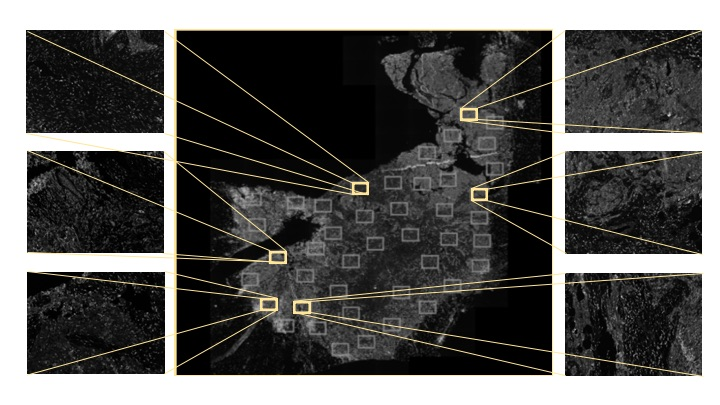
\includegraphics[width=\columnwidth]{doc/report/images/scan1.jpg}
  \caption{Example of a low resolution medical image with six high-resolution
snapshots. Middle: low-resolution of the whole slide with 45 snapshot positions
(small boxes). Left and Right: example of six high-resolution snapshots.}
  \vspace{-3mm}
  \label{fig:melanoma-scan}
\end{figure}


\section{State of the art}\label{sec:state-of-art}
\textbf{Survey the related work, giving credit where credit is
  due.} In the literature, several models have been proposed to perform super-resolution on medical images. We will survey them to get an idea what has already been done and from what we can take inspiration. A simple way to re-sample a low-resolution image to high-resolution is to apply interpolation (bicubic, bilinear, nearest neighbour, etc). Nevertheless, those can cause overshooting, clipping and images may be blurred. Thus, more elaborate models are provided, with the assumption that high-resolution images are made available. In ~\cite{zhang2019}, Zhang et al. suggest a method for fast single image super-resolution (FMISR) with three hidden layers in addition to a sub-pixel convolution layer and a mini-array. This model, they argue, improves the speed and quality of image reconstruction. Nonetheless, as it is used and trained on MRI and CT scans of the retinal macula, brain and bones, and thus are more a broad overview of those structures without cellular composition, it is not ideal for our melanoma stroma scans, which are more cell focused (\textbf{other way to formulate ?}). In ~\cite{nature2019}, Hongda Wang et al. present a deep-learning-enabled super-resolution model across different fluorescence microscopy modalities. Their method is based on training a generative adversarial network (GAN) to create super resolution total internal reflection fluorescence (TIRF) microscopy images of sub-cellular structures from diffraction-limited input images. Nevertheless, we have chosen not to follow a GAN structure because of their tendency to be unstable and their lengthy convergence time. \textbf{complete?}
  
 \begin{figure}[tbp]
  \centering
  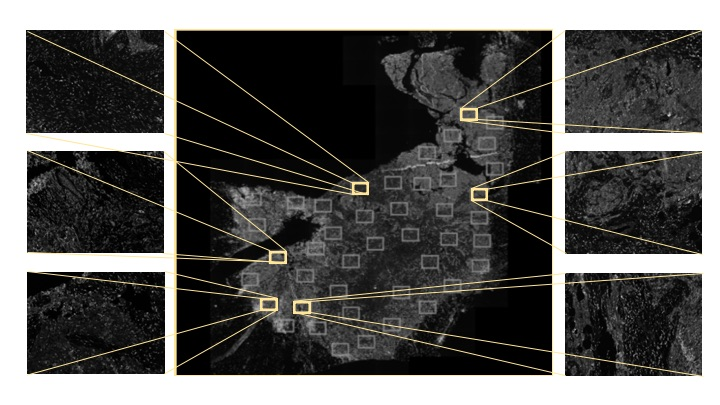
\includegraphics[width=\columnwidth]{doc/report/images/scan1.jpg}
  \caption{Example of a low resolution medical image with six high-resolution
snapshots. Middle: low-resolution of the whole slide with 45 snapshot positions
(small boxes). Left and Right: example of six high-resolution snapshots.}
  \vspace{-3mm}
  \label{fig:phenotypes}
\end{figure}


\section{Models and Methods}\label{sec:models-methods}
\subsection{The data}\label{subsec:data}
As previously mentioned, our data consists of 5-channel low-resolution raw .im3 files and 35-channel high-resolution snapshots. In Additionally, inForm outputs for each high-resolution patch its location, 3-channel phenotype images (see Figure~\ref{fig:phenotypes}), cell labelling data, and cell and tissue segmentation images. The phenotypes data included are: 
\begin{itemize}
    \item DAPI: blue-fluorescent DNA stain used for cell-center staining in fluorescence microscopy
    \item CD4: glycoprotein found on the surface of immune cells such as T lymphocytes. As previously stated in ~\cite{Carstens2017}~\cite{Bottomley2019}, knowledge of the distribution of immune cells in proximity to cancerous cells can give crucial information about patients survival and influence the choice of therapy.
    \item CD3: protein complex and T lymphocyte cell co-receptor.
    \item CD8: transmembrane glycoprotein that serves as a co-receptor for the T-cell receptor.
    \item FOXP3: protein involved in regulating the development and function of regulatory T lymphocyte cells.
    \item CK: cytokeratin, intermediate filaments forming the proteins that provide mechanical support for the cells. CKs are important markers for tumour cells. Primarily, metastases of a given carcinoma share a common cytokeratin pattern, which distinguishes them from other types of cancer, thus making it possible to distinguish between different tumors.
\end{itemize} 


\subsection{Method}
\textbf{ Describe your idea and how it was implemented to solve
  the problem.}
The models and methods
section should describe what was
done to answer the research question, describe how it was done,
justify the experimental design, and
explain how the results were analyzed.

The model refers to the underlying mathematical model or structure which 
you use to describe your problem, or that your solution is based on. 
The methods on the other hand, are the algorithms used to solve the problem. 
In some cases, the suggested method directly solves the problem, without having it 
stated in terms of an underlying model. Generally though it is a better practice to have 
the model figured out and stated clearly, rather than presenting a method without specifying 
the model. In this case, the method can be more easily evaluated in the task of fitting 
the given data to the underlying model.

The methods part of this section, is not a step-by-step, directive,
protocol as you might see in your lab manual, but detailed enough such
that an interested reader can reproduce your
work~\cite{anderson04,wavelab}.

The methods section of a research paper provides the information by
which a study's validity is judged.
Therefore, it requires a clear and precise description of how an
experiment was done, and the rationale
for why specific experimental procedures were chosen.
It is usually helpful to
structure the methods section by~\cite{kallet04methods}:
\begin{enumerate}
\item Layout the model you used to describe the problem or the solution.
\item Describing the algorithms used in the study, briefly including
  details such as hyperparameter values (e.g. thresholds), and
  preprocessing steps (e.g. normalizing the data to have mean value of
  zero).
\item Explaining how the materials were prepared, for example the
  images used and their resolution.
\item Describing the research protocol, for example which examples
  were used for estimating the parameters (training) and which were
  used for computing performance.
\item Explaining how measurements were made and what
  calculations were performed. Do not reproduce the full source code in
  the paper, but explain the key steps.
\end{enumerate}
 

\section{Results}\label{sec:results}
\textbf{Show evidence to support your claims made in the
  introduction.}
  Organize the results section based on the sequence of table and
figures you include. Prepare the tables and figures as soon as all
the data are analyzed and arrange them in the sequence that best
presents your findings in a logical way. A good strategy is to note,
on a draft of each table or figure, the one or two key results you
want to address in the text portion of the results.

\section{Discussion}\label{sec:discussion}
  \textbf{Discuss the strengths and weaknesses of your
  approach, based on the results. Point out the implications of your
  novel idea on the application concerned.}
  
\section{Summary}\label{sec:summary}
  \textbf{Summarise your contributions in light of the new
  results.}

\section*{Acknowledgements}
TO COMPLETE.

\newpage
\bibliographystyle{IEEEtran}
\bibliography{literature}

\end{document}